\documentclass[12pt,letterpaper]{article}
\usepackage[utf8]{inputenc}
\usepackage[spanish,mexico]{babel}
\usepackage{amsmath}
\usepackage{amsfonts}
\usepackage{amssymb}
\usepackage{amsmath}
\usepackage[lmargin=3cm,rmargin=3cm,tmargin=3cm,bmargin=3cm]{geometry}

\usepackage{hyperref}
\usepackage{graphicx}
\usepackage{float}


\begin{document}

\title{Actividad 5:  Movimiento armónico simple: Péndulo}
\author{Luisa Fernanda Orci Fernandez.}
\date{18 de Febrero del 2016}

\maketitle


\section*{Péndulo}
En esta actividad volvemos a retomar el tema de la actividad 1, el péndulo. Este es un sistema físico que puede oscilar bajo la acción de la gravedad. \\ 
Existen varios tipos de péndulos, algunos de ellos son el péndulo simple, el compuesto, el doble péndulo, el péndulo de torsión, el de Newton, entre otros. Uno de los usos que se le dan al péndulo es el de medir el tiempo, o medir la gravedad. \\

Matemáticamente el péndulo es muy complicado, pero se puede simplificar tomando en cuenta algunas suposiciones para facilitar su cálculom como por ejemplo, un péndulo simple con ángulos pequeños. \\

En esta actividad se nos solicitó un código que fuera capaz de resolver la ecuación de movimiento de un péndulo; $$ \frac{d^2\theta}{dt^2} + \frac{g}{l}\sin\theta = 0  $$, la cual es una ecuación diferencial de segundo orden.

\section*{Actividad}
Para poder llevar a cabo esta actividad, se nos proporcionó un código donde se resuelve esta ecuación para cualquien ángulo $theta$. Este lo obtuvimos de la página $ SciPy.org $, el código es el siguiente: 

\begin{verbatim}
import numpy as np
>>> def pend(y, t, b, c):
...     theta, omega = y
...     dydt = [omega, -b*omega - c*np.sin(theta)]
...     return dydt
...
>>> b = 0.25
>>> c = 5.0
>>> y0 = [np.pi - 0.1, 0.0]
>>> t = np.linspace(0, 10, 101)
>>> from scipy.integrate import odeint
>>> sol = odeint(pend, y0, t, args=(b, c))
>>> import matplotlib.pyplot as plt
>>> plt.plot(t, sol[:, 0], 'b', label='theta(t)')
>>> plt.plot(t, sol[:, 1], 'g', label='omega(t)')
>>> plt.legend(loc='best')
>>> plt.xlabel('t')
>>> plt.grid()
>>> plt.show()
\end{verbatim}
Y la gráfica fue la siguiente: 
\begin{center}
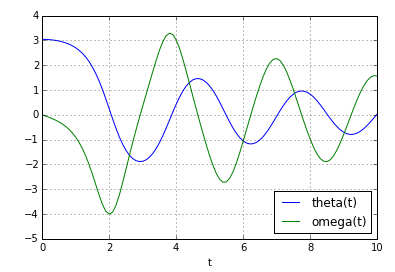
\includegraphics[scale=0.7]{act5.png}
\end{center}

Este código lo modificamos de la siguiente manera: 

\begin{itemize}
\item Primeramente se definió la ecuación: $ theta''(t) + b*theta'(t) + c*sin(thetha(t)) = 0 $, donde las tildes son la primera y segunda derivada.
\item Después convertimos esta ecuación en un sistema de ecuaciones de primer orden, donde la velocidad angular omega es $ (t) = theta'(t) $, después obtuvimos el sistema donde $ theta'(t) = omega(t) $ y quedó de la siguiente forma: $$ omega'(t) = -b*omega(t)-c*sin(theta(t)) $$.
\item El vector $y$ quedó como $[theta, omega]$.
\item Consideramos que el péndulo estaba con posición vertica con $y0 = [np.pi-0.1, 0.0]$
\item Después se generó una solución de 101 muestras uniformemente espaciadas en un intervalo $ 0 <= t <= 10 $.
\item Para generar la solución llamamos a $odeneit$, y le dimos los parámetros $b$ y $c$ utilizando $args$.
\end{itemize}

Quedó de la siguiente manera:

\begin{verbatim}
#Modifiacion, friccion = 0, theta = pi-0.1, c = 5
def pend(y, t, b, c):
    theta, omega = y
    dydt = [omega, -b*omega - c*np.sin(theta)]
    return dydt
    
b = 0.0
c = 5.0
y0 = [np.pi-0.1, 0.0]
t = np.linspace(0, 100, 101)
    
from scipy.integrate import odeint
sol = odeint(pend, y0, t, args=(b, c))
import matplotlib.pyplot as plt
   
plt.plot(t, sol[:, 0], 'b', label='theta(t)')
plt.plot(t, sol[:, 1], 'g', label='omega(t)')
plt.legend(loc='best')
plt.xlabel('t')
plt.grid()
plt.show()

\end{verbatim}
y la gráfica fue: 

\begin{center}
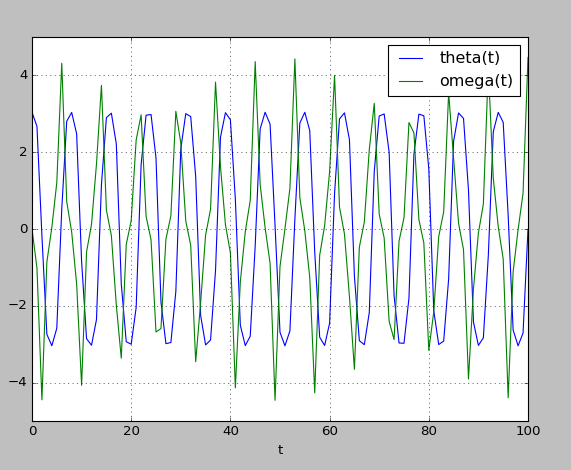
\includegraphics[scale=0.6]{act5codigo1.png}

\end{center}

\section{Resultados}
\subsection*{Modificación 1}

En este caso la única modificación realizada fue al ángulo, se utilizó un ángulo de $\frac{\pi}{4}$: 

\begin{verbatim}
#Caso 1, friccion = 0, theta = pi/4, c = 5
def pend(y, t, b, c):
    theta, omega = y
    dydt = [omega, -b*omega - c*np.sin(theta)]
    return dydt
    
b = 0
c = 5.0
y0 = [np.pi/4, 0.0]
t = np.linspace(0, 100, 101)
    
from scipy.integrate import odeint
sol = odeint(pend, y0, t, args=(b, c))
import matplotlib.pyplot as plt
   
plt.plot(t, sol[:, 0], 'b', label='theta(t)')
plt.plot(t, sol[:, 1], 'g', label='omega(t)')
plt.legend(loc='best')
plt.xlabel('t')
plt.grid()
plt.show()
\end{verbatim}

y la gráfica fue: 

\begin{center}
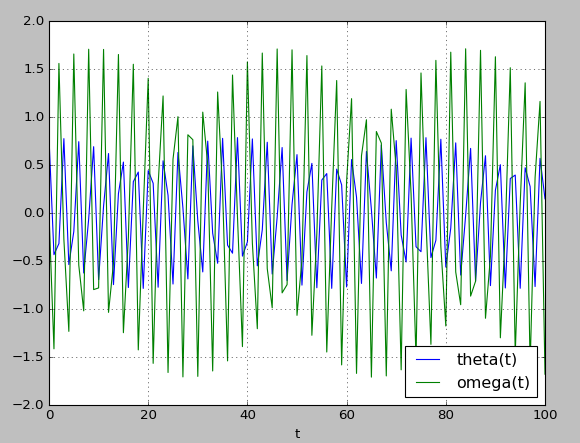
\includegraphics[scale=0.6]{act5caso1.png}
\end{center}

\newpage

\subsection*{Modificación 2}
Esta vez si agregamos fricción y se tomó un ángulo de $\frac{\pi}{4}$

\begin{verbatim}
#Caso 2, friccion = .5, theta = pi/4, c = 5
def pend(y, t, b, c):
    theta, omega = y
    dydt = [omega, -b*omega - c*np.sin(theta)]
    return dydt
    
b = 0.5
c = 5.0
y0 = [np.pi/4, 0.0]
t = np.linspace(0, 100, 101)
    
from scipy.integrate import odeint
sol = odeint(pend, y0, t, args=(b, c))
import matplotlib.pyplot as plt
   
plt.plot(t, sol[:, 0], 'b', label='theta(t)')
plt.plot(t, sol[:, 1], 'g', label='omega(t)')
plt.legend(loc='best')
plt.xlabel('t')
plt.grid()
plt.show()
\end{verbatim}
La gráfica que resultó fue:
\begin{center}
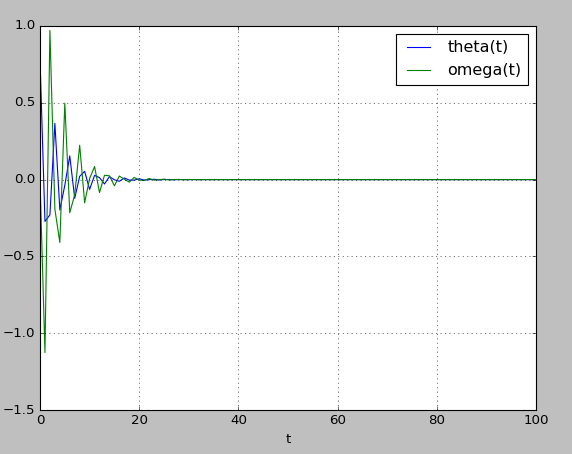
\includegraphics[scale=0.6]{act5caso2.png}
\end{center}

\newpage

\subsection*{Modificación 3}
Esta vez si agregamos fricción y se tomó un ángulo de $\frac{\pi}{4}$ pero esta vez se modific[o la longuitud del péndulo.

\begin{verbatim}
#Caso 3, friccion = 0, theta = pi/4, c = .25
def pend(y, t, b, c):
    theta, omega = y
    dydt = [omega, -b*omega - c*np.sin(theta)]
    return dydt
    
b = 0.0
c = .25
y0 = [np.pi/4, 0.0]
t = np.linspace(0, 100, 101)
    
from scipy.integrate import odeint
sol = odeint(pend, y0, t, args=(b, c))
import matplotlib.pyplot as plt
   
plt.plot(t, sol[:, 0], 'b', label='theta(t)')
plt.plot(t, sol[:, 1], 'g', label='omega(t)')
plt.legend(loc='best')
plt.xlabel('t')
plt.grid()
plt.show()
\end{verbatim}
La gráfica que resultó fue:
\begin{center}
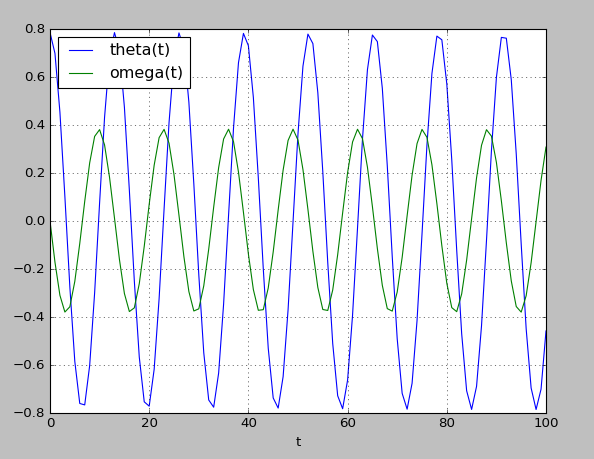
\includegraphics[scale=0.6]{act5caso3.png}
\end{center}

\newpage

\subsection*{Modificación 4}
Aquí hubo modificación en la fricción, el ángulo y la longuitud.

\begin{verbatim}
#Caso 4, friccion = .6, theta = pi/4, c = 5
def pend(y, t, b, c):
    theta, omega = y
    dydt = [omega, -b*omega - c*np.sin(theta)]
    return dydt
    
b = 0.6
c = 5.0
y0 = [np.pi/4, 0.0]
t = np.linspace(0, 100, 101)
    
from scipy.integrate import odeint
sol = odeint(pend, y0, t, args=(b, c))
import matplotlib.pyplot as plt
   
plt.plot(t, sol[:, 0], 'b', label='theta(t)')
plt.plot(t, sol[:, 1], 'g', label='omega(t)')
plt.legend(loc='best')
plt.xlabel('t')
plt.grid()
plt.show()
\end{verbatim}
La gráfica final quedó así:

\begin{center}
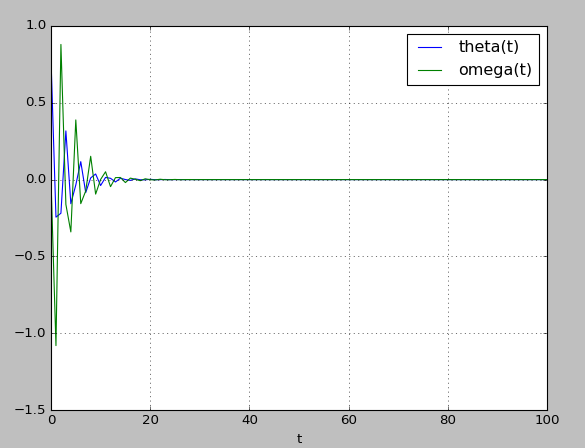
\includegraphics[scale=0.6]{act5caso4.png}
\end{center}

\section*{Conclusión}
Esta actividad resultó muy interesante ya que tuvimos la oportunidad de modelar un fenómeno físico y como estudiante de la Licenciatura en Física, esto resultará de mucha ayuda en un futuro. De igual manera resulta muy útil el entender como construir un programa que nos ayude con esto. 

\begin{thebibliography}{widestlabel}
	\bibitem{w} Wikipedia, https://es.wikipedia.org/wiki/Pendulo
	\bibitem{s} Scipy, http://scipy.github.io/devdocs/generated/scipy.integrate.odeint.html
\end{thebibliography}


\end{document}